%%% ---------------
%%% PREAMBLE
%%% ---------------
\documentclass[french,11pt]{article}

% Define geometry (without using the geometry package)
\usepackage[a4paper]{geometry}
\geometry{landscape, twocolumn, textwidth=27.5cm, textheight=19.5cm, columnsep=20mm}

%\frenchspacing						% better looking spacing

% Call packages we'll need
\usepackage{graphicx}				% images
\usepackage{multicol}
\usepackage{multirow}
\usepackage{url}					% clickable links
\usepackage{marvosym}				% symbols
\usepackage{wrapfig}				% wrapping text around figures
\usepackage{fontspec}			% font encoding
\usepackage{xunicode}
\usepackage{phonenumbers}
\usepackage[hidelinks]{hyperref}
\usepackage{ragged2e}
\usepackage{titlesec}
\usepackage{framed}
%\usepackage[default]{raleway}
\usepackage{tocvsec2}
% Customize (header and) footer
\usepackage{fancyhdr}
\usepackage{enumitem}
\usepackage{fontawesome}
\usepackage{lipsum}
\usepackage{babel}
%\usepackage{currency}
%\pagestyle{fancy}
\pagestyle{empty}
\setmainfont{Carlito}

%\newfontfamily\headingfont[]{Arial}
%\titleformat*{\section}{\Large\bfseries\sffamily}
%\titleformat*{\section}{\Large\headingfont}

%\renewcommand{\headrulewidth}{0.0pt}	% no bar on top of page
%\renewcommand{\footrulewidth}{0.4pt}	% bar on bottom of page

%%% ---------------
%%% DEFINITIONS
%%% ---------------

% Define separators

% Define Title en News input
\newcommand{\JournalName}[1]{%
		\begin{center}
			%\Huge \usefont{T1}{augie}{m}{n}
            \Large \usefont{T1}{augie}{m}{n}
			#1%
		\end{center}
		\par \normalsize \normalfont}

\newcommand*{\chants}{../chants}
\newcommand*{\messe}{../messe_david_julien}
\newcommand*{\pu}{../pu}
\newcommand*{\psaumes}{../psaumes}
\newcommand*{\footer}{..}

%\DefineCurrency{EUR}{name={euro}, plural={euros}, symbol={\euro}, iso={EUR}, kind=iso}

\newcommand{\NewsItem}[1]{%
\vspace{3pt}
\underline{\textbf{#1}}
	%	%\usefont{T1}{augie}{m}{n}
	%	\large \textbf{#1} %\vspace{3pt}
   %     %\Large #1 \vspace{4pt}
	%	%\par
   %     \normalsize \normalfont
		  }

\newcommand{\NewsAuthor}[1]{%
			\hfill by \textsc{#1} \vspace{4pt}
			\par \normalfont}
%\sisetup{locale=FR}
%\sisetup{group-minimum-digits=3}

\graphicspath{{../images/}}

%pas de numérotation des sections
\setsecnumdepth{none}
\setlength{\parindent}{0pt}
%%% ---------------
%%% BEGIN DOCUMENT
%%% ---------------
\begin{document}

\NewsItem{CHANT D'ENTRÉE}\\
	Entrez, Dieu est en attente,
Sa maison est un lieu pour la paix.
Goûtez, Dieu est en partage,
Sa table est un lieu pour se donner.

1.
Vous êtes le peuple de Dieu,
Pierres vivantes de son église,
Traces brûlantes de son passage,
Jetant les grains de l'évangile.

2.
Vous êtes le peuple de Dieu,
Marques vivantes de son visage,
Signes visibles de sa tendresse,
Portant les fruits de l'évangile.

%3.
%Vous êtes le peuple de Dieu,
%Fêtes vivantes de sa promesse,
%Pages ardentes de sa parole,
%Jouant les mots de sa musique. 


\NewsItem{PRÉPARATION PÉNITENTIELLE}\\
	Seigneur, prends pitié. Seigneur prends pitié, Seigneur, prends pitié\\
Ô Christ, prends pitié. ô Christ prends pitié, o Christ, prends pitié.\\
Seigneur, prends pitié. Seigneur, prends pitié Seigneur, prends pitié


\NewsItem{GLORIA}\\
	\begin{itemize}
\item[R/] 
Gloire à Dieu, au plus haut des cieux, et paix sur la terre, aux hommes qu'il aime. (bis)
\item[1.]
Nous te louons, nous te bénissons, nous t’adorons, nous te glorifions, nous   
      te rendons grâce pour ton immense gloire. Seigneur Dieu, Roi du ciel, Dieu 
      le Père tout puissant. R/
\item[2.]
Jésus-Christ, Seigneur Fils unique, Agneau de Dieu, le Fils du Père, toi qui 
      enlèves le péché du monde, reçois nos prières. Toi qui es assis à la droite  
      du Père, prends pitié de nous. R/
\item[3.]
Car toi seul es saint, toi seul es Seigneur, toi seul es le Très Haut : 
      Jésus-Christ, avec le Saint Esprit, dans la gloire de Dieu le Père. R/
\end{itemize}




% -----
\NewsItem{1\iere{} LECTURE} Is 66, 18-21
% -----

\NewsItem{PSAUME}
Ps 116 (117), 1, 2

\textbf{
Allez dans le monde entier.
Proclamez l’Évangile.}

\smallskip

Louez le Seigneur, tous les peuples ;\\
fêtez-le, tous les pays !

\smallskip

Son amour envers nous s’est montré le plus fort ;\\
éternelle est la fidélité du Seigneur !



% -----
\NewsItem{2\ieme{} LECTURE} He 12, 5-7.11-13

\NewsItem{ACCLAMATION}
Alleluia \emph{messe du Peuple de Dieu}


\NewsItem{ÉVANGILE} Lc 13, 22-30

\NewsItem{HOMÉLIE}

\NewsItem{PROFESSION DE FOI}
%\textbf{Je crois en Toi Père, Fils et Esprit. J’ai confiance en Toi, Tu es mon ami.}


\begin{tabular}{p{0.5\columnwidth} p{0.5\columnwidth}}
1 - Père Créateur de vie, nous sommes tes enfants, Tu nous donnes la vie, 
  Toi qui nous aimes tant.
&
2 - Jésus né de Marie, Tu es le Fils de Dieu. Tu nous 
  donnes Ta vie comme un cadeau précieux.
\\
3 - Et Toi Esprit de Dieu, Tu nous 
  donnes Ta force, un souffle silencieux nous unit, nous renforce.
&
4 - Je crois 
 que je grandis en Te confiant ma vie, ma famille, mes amis, au nom du Père, 
  du Fils et de l’Esprit.\newline
  Amen. Amen. Amen. 
\end{tabular}




%\newpage

\NewsItem{PRIÈRES UNIVERSELLES}
Sauveur du monde attire à toi les hommes


\NewsItem{OFFERTOIRE}

\NewsItem{PRIÈRES SUR LES OFFRANDES}
\textit{Nous nous levons et nous répondons : }
Que le Seigneur reçoive de vos mains ce sacrifice à la louange et à la gloire
de Son nom, pour notre bien et celui de toute l’Église.

\NewsItem{SANCTUS}
Le Seigneur est Saint ! Le Seigneur est Saint ! Le Seigneur est Saint !
Le Seigneur est notre Dieu, Le Seigneur est notre Père. Il règne dans les cieux, qu’Il règne sur la terre.


\NewsItem{ANAMNÈSE}
Christ est venu, Christ est né, Christ a souffert, Christ est mort, 
Christ est ressuscité, Christ est vivant,
Christ reviendra, Christ est là,
Christ reviendra, Christ est là.


\NewsItem{NOTRE PÈRE}

\NewsItem{AGNUS} \\
Agneau de Dieu Qui enlèves le péché du monde, Prends pitié de nous !  Prends pitié de nous ! (bis) \\
Agneau de Dieu Qui enlèves le péché du monde, Donne-nous la paix !  Donne-nous la paix !


\NewsItem{COMMUNION}
\emph{En mémoire du Seigneur}

\textbf{
Pour un monde nouveau,
Pour un monde d’amour \dots \\
Et que viennent les jours
De justice et de Paix !
}

\begin{tabular}{p{0.5\columnwidth} p{0.5\columnwidth}}
1.
En mémoire du Seigneur \newline
Qui nous a rompu le pain, \newline
En mémoire du Seigneur \newline
Nous serons le pain rompu.
&
2.
En mémoire du Seigneur \newline
Qui nous a donné son sang, \newline
En mémoire du Seigneur \newline
Nous serons le sang versé.
\\
3.
En mémoire du Seigneur \newline
Qui a fait de nous son corps, \newline
En mémoire du Seigneur \newline
Nous serons son corps livré.
&
4.
En mémoire du Seigneur \newline
Tout le pain soit partagé ! \newline
En mémoire du Seigneur \newline
Tous les pauvres soient comblés ! 
\end{tabular}


\NewsItem{ANNONCES PAROISSIALES}


\NewsItem{CHANT D'ENVOI}\\
\begin{tabular}{p{0.5\columnwidth} p{0.5\columnwidth}}
1.
L´amour a fait les premiers pas,\newline
L'amour a préparé la noce.\newline
Les invités ne viennent pas.\newline
L'amour a fait les premiers pas.\newline
Les places vides sont offertes\newline
À ceux que l´on n'attendait pas,\newline
L'amour a fait les premiers pas.\newline
Il nous adresse la parole,\newline
Il nous invite à son repas,\newline
L'amour a fait les premiers pas,\newline
L'amour a fait les premiers pas.
&
2.
L'amour a pris la liberté\newline
De négliger les convenances.\newline
Il s´est chargé de l'étranger.\newline
L'amour a pris la liberté.\newline
Il laisse les brebis fidèles\newline
Pour celle qui s'est égarée.\newline
L'amour a pris la liberté.\newline
Il attendait l´enfant prodigue.\newline
Il nous invite à le fêter.\newline
L´amour a pris la liberté,\newline
L´amour a pris la liberté.
\end{tabular}
%3
%L'amour efface le passé.
%Aucun n´osa jeter la pierre.
%Et tous les yeux se sont baissés.
%L´amour efface le passé.
%Il a vu l'homme dans sa lèpre.
%Il n´a pas peur de l'embrasser.
%L'amour efface le passé.
%Il nous redonne une autre chance,
%Il nous invite à pardonner.
%L´amour efface le passé,
%L´amour efface le passé.
%4
%L'amour annonce l'avenir.
%Il fait renaître de la cendre
%La flamme qui allait mourir.
%L'amour annonce l'avenir.
%Il donne jour à l´espérance.
%Il fait renaître le désir.
%L´amour annonce l'avenir.
%Il nous redonne sa confiance.
%Il nous invite à repartir.
%L'amour annonce l'avenir,
%L'amour annonce l'avenir. 


\newpage


\NewsItem{Intentions de messe}
\begin{itemize}
\item[\Cross] Célestin NDIOGOYE
\item[\Cross]Benoit NDIOGOYE
\item[\Cross]Pierre NDIOGOYE
\item[\Cross]Michel NDIOGOYE
\item[\Cross]Léopold NDIOGOYE
\item[\Cross]Charlotte NDIOGOYE
\end{itemize}

\NewsItem{Informations paroissiales}

\begin{tabular} {lcp{9cm}}
\multicolumn{3}{c}{\textbf{Saint Jean-Baptiste} } \\ \hline
%Mardi    & 01 juillet  & Vêpres 18h15. Messe 18h30 \\ \hline
Jeudi    & 28 août &
Exposition du Saint Sacrement à 16h00. Adoration. Salut au Saint Sacrement à 18h15. Messe à 18h30 
 \\ \hline
Vendredi & 29 août & Laudes 08h45. Messe 09h00 \\ \hline
Samedi   & 30 août & Messe anticipée 18h00 \\ \hline
%Dimanche & & Pas de messe \\ \hline
\multicolumn{3}{c}{\textbf{Sainte Croix} } \\ \hline
%Mercredi & 02 juillet  & Messe 09h00.
%\newline \Cross{} \textbf{Enterrement}  14h30 Marie-Claire Noël \\ \hline
Dimanche  & 31 août & Messe 10h00\\ \hline
%\multicolumn{3}{c}{\textbf{Résidence Landsberg (3 rue Jean Monnet)} } \\ \hline
%Mercredi & 02 juillet : & Messe 10h45 \\ \hline
\end{tabular}

\begin{framed}
\begin{tabular} {lcp{7cm}}
\multicolumn{3}{c}{\textbf{Saint Jean-Baptiste} } \\
\multicolumn{3}{l}{ Du 06 juil. au 14 sept. : pas de messe le dimanche } \\
%Vendredi & 01 août & 08h45 Laudes. Pas de messe. \\
\multicolumn{3}{c}{\textbf{Sainte Croix} } \\
\multicolumn{3}{l}{ Du 06 juil. au 14 sept. : \textbf{messe unique} le dimanche à Sainte Croix à 10h00.} \\
Dimanche & 14 sept. & Messe de rentrée 10h00 \\
Dimanche & 14 sept. &  Barbecue 12h00 - 15~euros. \newline
 Inscription avant le 07 sept. auprès de Bernard Braun \texttt{bernardbrstr@gmail.com} ou \texttt{06~83~82~52~50}\\
%\multicolumn{3}{c}{\textbf{Foyer Oberlin} } \\
%\multicolumn{3}{c}{\textbf{Résidence Landsberg (3 rue Jean Monnet)} } \\
%Mercredi & 09 juillet & Messe 10h45 \\ \hline
\end{tabular}
\end{framed}

\NewsItem{Répétitions des chorales}
\begin{description}
\item[Chorales paroissiales] : reprise le vendredi 05 septembre (20h15 à Ste Croix)
%\item[Chorales paroissiales] : vendredi 20h15 à Sainte Croix
\end{description}

\begin{framed}
\textbf{Presbytère St Jean-Baptiste}
%2 rue de l'école 67380 Lingolsheim 03 88 78 16 45 \\
2 rue de l'école 67380 Lingolsheim \phonenumber[country=FR]{0388781645} \\
\textbf{Permanence} Lun. au Jeu. : 09h30-12h00 et 15h-18h. Ven. 16h-18h00. Sam. 09h30-12h00. \\
\textbf{Courriels} \texttt{nddessables@hotmail.com}, \texttt{danielette67380@gmail.com}

%\textbf{Caritas} Vestiaire ouvert le mardi de 14h à 16h

\texttt{https://stjeanbaptistelingo.fr} \hfill \faFacebook Catho Lingo \hfill \faInstagram @catho\_lingo
\end{framed}



\newpage

\JournalName{Communauté de Paroisses de Lingolsheim \\
\normalsize \textit{Notre Dame des Sables}
%\\ \large \'{E}glise Saint Jean-Baptiste
\\  \normalsize \textit{21\ieme{} dimanche du Temps Ordinaire - C}
\\ \large Dimanche 24 août 2025}
%\noindent\HorRule{3pt} \\[-0.75\baselineskip]
%\HorRule{1pt}
% -----

% Front article
% -----
%\vspace{0.5cm}
%	\SepRule
%\vspace{0.5cm}

%\begin{center}
\begin{minipage}[h]{1.0\linewidth}
\setlength{\parindent}{1em}
 \begin{center}
 \textbf{
 %\dots
\og 
Rentrée Pastorale 2025-2026
 \fg{}
 %\dots
 }
 \end{center}

%\begin{wrapfigure}{l}{1.3cm}
%\vspace{-0.4cm}
%	\includegraphics[scale=1.0]{../images/lazarre}
%\end{wrapfigure}
Une nouvelle rentrée pastorale qui nous réjouit tous. En effet, après un temps de répit, il nous revient de mettre en marche la machine de nos activités pastorales.

Au début de cette nouvelle année pastorale, je souhaite vous redire toute ma joie de vous retrouver pour continuer la mission qui m’est assignée dans notre communauté de paroisses. Et comme chaque année, nous mettrons l’accent en premier lieu sur la vie catéchétique des enfants et des adolescences, l’animation liturgique, la création d’une troisième chorale, la visite aux malades et dans notre maison de retraite ( \emph{Résidence du Parc}), l’accueil et l’accompagnement en vue de baptêmes,  du catéchuménat des adultes, des mariages, l’encadrement  des servants d’autel, l’entretien de notre église pour la rendre  accueillante, avec ces innombrables petits gestes de service qui jalonnent l’existence ; tout cela nous aidera à vivre une véritable dimension ecclésiale.

Je voudrais vous remercier de tout cœur, vous tous qui êtes des membres vivants et actifs de la communauté paroissiale que nous formons, véritable artisans de l’évangélisation ordinaire. Mon souhait pour la vie de notre communauté de paroisses est que nous arrivions toujours plus à nous ouvrir et à nous connaître les uns les autres, à nous apprécier dans ce que nous sommes et vivons.

L’année dernière, avec toutes les entités de nos deux paroisses, nous avons eu différentes propositions, activités et invitations qui ont favorisées l’\textbf{Unité et l’ouverture} qui constituaient notre thème pastoral. Ne manquons pas cette année ces moments simples et conviviaux qui permettent de tisser des liens gratuits, profonds et tout simplement chrétiens.

\begin{wrapfigure}{l}{1.2cm}
\vspace{-0.4cm}
	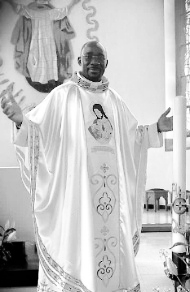
\includegraphics[scale=1.20]{../images/standing_daniel}
\end{wrapfigure}
Cette année nous porterons ensemble cette rentrée dans le cœur de chacun avec nos \textbf{jeunes pro}. Chacun à son rythme, selon ses possibilités et ses réalités mais avec un seul et même objectif : l’accomplissement de nos activités communautaires. Présentons également notre rentrée paroissiale au Christ. Et continuons notre chemin pour la mise en œuvre de notre projet paroissial autour de ce principal thème : \textbf{\og Avec notre jeunesse bâtissons une communauté plus dynamique, rayonnante et missionnaire\fg{}.}

	Que cette rentrée pastorale nous aide à prendre des résolutions nécessairement pour plonger à frais nouveaux dans la parole et être des disciples crédibles de l’évangile.


\begin{flushright}
Bonne rentrée pastorale à toutes et à tous !
\textit{Père  Daniel  ETTÉ}
\end{flushright}


\end{minipage}
%\end{center}
% -----
\end{document}
